\section{Степенные ряды. Теорема о сходимости ряда при меньших аргументах. Радиус и круг сходимости. Формула Коши–Адамара. Примеры}
\begin{conj}
    Степенным рядом называется ряд вида $\sum\limits_{n=0}^\infty a_n(z - z_0)^n$, где $a_n, z, z_0 \in \C$.
\end{conj}
\begin{notice}
    Сделав замену $w := z - z_0$, получаем ряд $\sum\limits_{n=0}^\infty a_n w^n$, в котором $z_0 = 0$. 
    Зачастую именно такая форма более удобна, а к общей форме можно легко перейти сдвигом.
\end{notice}

\vspace*{5mm}

\begin{theorem} (Теорема Абеля)

    Если $\sum\limits_{n=0}^\infty a_n z^n$ сходится при $\widetilde{z} \neq 0$, то он абсолютно сходится при $|z| < |\widetilde{z}|$.    
\end{theorem}
\begin{proof}
    Если ряд $\sum\limits_{n=0}^\infty a_n (\widetilde{z})^n$ сходится, у нас должно выполняться необходимое условие сходимости: $a_n(\widetilde{z})^n \to 0$.
    Значит, $a_n(\widetilde{z})^n$ ограничены: $|a_n(\widetilde{z})^n| \leqslant M$. 
    Тогда при $|z| < |\widetilde{z}|$ наш ряд ограничен геометрической прогрессией:
    \begin{gather*}
        |a_nz^n| = |a_n\widetilde{z}^n| \cdot \left| \frac{z}{\widetilde{z}} \right|^n \leqslant M \left|\frac{z}{\widetilde{z}} \right|^n
    \end{gather*}
    Она является сходящейся, поэтому наш ряд сходится по признаку сравнению.
\end{proof}

Таким образом, данная теорема утверждает, что если ряд сходится в какой-то точке $z_0$, то отметив ее на комплексной плоскости, мы получим, что во всех точках, лежащих внутри круга с радиусом равным $|z_0|$, ряд будет сходиться.

Отметим одно очевидное следствие.

\begin{follow}
    Если $\sum\limits_{n=0}^\infty a_n z^n$ расходится при $z_0 \neq 0$, то он расходится и при $|z| > |z_0|$.
\end{follow}
\begin{proof}
    От противного: если бы он сходился при $z$, то по предыдущей теореме сходился бы и при $z_0$.
\end{proof}

\vspace*{5mm}

Все это наталкивает нас на мысль, что существует такой круг, что внутри него ряд сходится, а вне -- расходится.
Определим это формально.

\begin{conj}
    Радиус сходимости степенного ряда $\sum\limits_{n=0}^\infty a_n z^n$ -- это такое число $R \in [0, +\infty]$, что $\forall z : |z| < R$ ряд сходится, а $\forall z : |z| > R$ ряд расходится.
\end{conj}

\begin{conj}
    Круг сходимости степенного ряда $\sum\limits_{n=0}^\infty a_n (z - z_0)^n$ -- открытый круг радиуса $R$ (радиус сходимости) в точке $z_0$.
\end{conj}

\begin{center}
    % 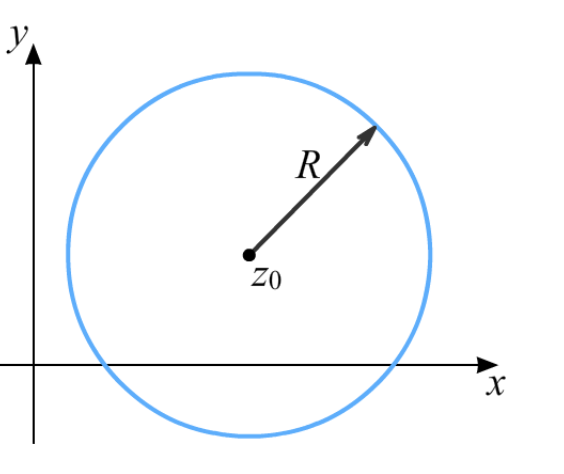
\includegraphics[scale=0.4]{circle.png}    
    \begin{tikzpicture}[thick]
        % Axes
        \draw[-latex,name path=xaxis] (-0.5,0) -- (5,0) node[above]{\large $x$};
        \draw[-latex] (0,-1) -- (0,4)node[right]{\large $y$};;
        
        \draw (2.5,1.5) node[circle,draw, inner sep=0.5pt,label=below:$z_0$](z0) {};
        \draw (2.5,1.5) [cyan] circle (3*pi/5);
        \draw[-stealth] (z0) -- (3.61, 3) node[midway,above]{$R$};
    \end{tikzpicture}
\end{center}

\begin{notice}
    Во всех точках круга сходимости ряд сходится. 
    Вне замыкания круга сходимости ряд расходится.
    Про границу мы ничего утверждать не можем. 
\end{notice}

\vspace*{10mm}

Давайте поймем, что любой степенной ряд имеет радиус сходимости.

\begin{theorem} (Формула Коши-Адамара)
    Всякий степенной ряд имеет радиус сходимости, причем его можно посчитать по формуле:
    \begin{gather*}
        R = \frac{1}{\overline{\lim\limits_{n \to \infty}} \sqrt[n]{|a_n|}}
    \end{gather*}
\end{theorem}
\begin{proof}
    Применим к ряду $\sum\limits_{n = 0}^\infty a_n z^n$ признак Коши, а именно, посчитаем 
    \begin{gather*}
        q^* = \overline{\lim\limits_{n \to \infty}} \sqrt[n]{|a_nz^n|}
    \end{gather*}
    (Вообще в признаке Коши под корнем нет модуля, но добавить его это законно, так как если сходится абсолютно, то сходится и обычно, а если абсолютно расходится, то по признаку Коши нет необходимого условия сходимости, то есть и обычно расходится.)

    Распишем $q^*:$ \[ q^* = \overline{\lim_{n \to \infty}} \sqrt[n]{|a_nz^n|} = \overline{\lim_{n \to \infty}} (\sqrt[n]{|a_n|} \cdot |z|) = |z| \cdot \overline{\lim_{n \to \infty}} \sqrt[n]{|a_n|}   \]
    Тогда согласно признаку Коши: \begin{itemize}
        \item Если $q^* < 1$, то ряд сходится $\Rightarrow$ если $|z| < \frac{1}{\overline{\lim\limits_{n \to \infty}} \sqrt[n]{|a_n|}}$, то ряд сходится.
        \item Если $q^* > 1$, то ряд сходится $\Rightarrow$ если $|z| > \frac{1}{\overline{\lim\limits_{n \to \infty}} \sqrt[n]{|a_n|}}$, то ряд сходится.
    \end{itemize}
    Это и говорит нам о том, что $R = \frac{1}{\overline{\lim\limits_{n \to \infty}} \sqrt[n]{|a_n|}}$ -- радиус сходимости.
\end{proof}

\begin{notice}
    Мы попутно поняли, что внутри круга сходимости ряд абсолютно сходится.
\end{notice}

\vspace*{7mm}
Поприменяем данную формулу на простых примерах.

\begin{examples}
    \begin{enumerate}
        \item $\sum\limits_{n=0}^\infty n!z^n$. 
        По формуле $R = \frac{1}{\overline{\lim\limits_{n \to \infty}} \sqrt[n]{n!}}$. 
        Так как предел этой последовательности существует, мы можем убрать знак верхнего предела: 
        \begin{gather*}
            R = \frac{1}{\lim\limits_{n \to \infty} \sqrt[n]{n!}} = \frac{1}{\lim\limits_{n \to \infty} (\frac{n}{e}\sqrt[2n]{2\pi n})} = \frac{1}{+\infty} = 0
        \end{gather*}
        $\Longrightarrow$ ряд сходится только в 0.
        \item $\sum\limits_{n=0}^\infty \frac{z^n}{n!}$. 
        По формуле $R = \frac{1}{\overline{\lim\limits_{n \to \infty}} \sqrt[n]{1/n!}}$.
        Опять же можем убрать верхний предел: 
        \begin{gather*}
            R = \frac{1}{\lim\limits_{n \to \infty} \sqrt[n]{1/n!}} = \lim\limits_{n \to \infty} \sqrt[n]{n!} = +\infty
        \end{gather*}
        $\Longrightarrow$ ряд сходится при всех $z \in \C$.
        \item $\sum\limits_{n=0}^\infty \frac{z^n}{n^p}$, где $p \in \R$.
        По формуле (сразу заменяем на обычный предел): 
        \begin{gather*} 
            R = \frac{1}{\lim\limits_{n \to \infty} \sqrt[n]{1/n^p}} = \lim\limits_{n \to \infty} \sqrt[n]{n^p} = 1
        \end{gather*}
        
        $\Longrightarrow$ ряд сходится при $|z| < 1$ и расходится при $|z| > 1$.

        Этот пример также демонстрирует тот факт, что на границе круга ряд может как сходиться, так и расходиться: \begin{itemize}
            \item Если $p = 2$, то $|\frac{z}{n^2}| \leqslant \frac{1}{n^2}$ при $|z| \leqslant 1 \Rightarrow$ ряд сходится при $|z| \leqslant 1$.
            \item Если $p = 1$ и $z = 1$, то ряд расходится, так как является гармоническим.
            \item Если $p = 1$ и $z = -1$, то ряд сходится, так как является рядом Лейбница.
            \item Если $p = 0$, то при $|z| = 1$ ряд расходится, так как $|z| \nrightarrow 0$.
        \end{itemize}
    \end{enumerate}    
\end{examples}
